\chapter{Influencing Factors on Transit Ridership at Station-to-Station Level}
\markright{CHAPTER 5}

% 待修正,再稍微补充一点,有点短感觉。两段话差不多
\section{Introduction}
% background
\subsection{Background}
%
Urban rail transit is a type of high-capacity public transport generally found in urban areas. Because of the rapid, punctual and environment-friendly features, the urban rail transit is becoming one of the most important travel modes in modern cities. With the popularity of the urban rail transit in modern cities and the emphasis on sustainable development, the concept of TOD (Transit Oriented Development) is put forward, intended to build the compact city \cite{calthorpe1993next}. Many cities around the world have adopted the policy of giving priority to the development of public transport for decreasing the share of motorized travel and increasing the willingness of using public transit. For policymakers, how to grasp the relation between land-use and transit ridership has become an important issue that they must face.

%
Although there have been lots of research on the relationship between land-use and transit ridership, most of them are conducted from the perspective of the single station. The transit ridership of a station, however, should be affected not only by the elements around that station, but also be affected by the transit ridership of other stations, since all the stations are running in the same system.  Once the circumstance within catchment area changes, obviously, the ridership of this station will change as well. But the increased part of passengers will be transported to other stations, thus every station connected to that station will also have an increase in ridership. 

% why focus on the ridership at station-to-station level
\subsection{Research purpose}
%
Some researchers have discussed on the issue of inter-urban transit demand at station-to-station level \cite{wardman1997inter,jones1983demand}, nevertheless, restricted by the difficulties in collecting data at station-to-station level, few studies focused on intra-urban transit demand \cite{choi2012analysis}. Even now, the transit ridership forecasting at station-to-station level is still difficult due to the complex interaction among stations. 

Based on this realistic background, this study will focus on the relation among stations from the perspective of land-use. But rather than making the prediction of transit ridership between station and station, this study tries to explain what factors of land-use can influence the choice of destination station for passengers. 

\section{Review}
%
Until now, there are many studies focusing on the relationship between various factors and transit ridership. Most of the studies are based on regression model and conducted from the view of station-level, the transit ridership is thought to be affected by the circumstance surrounding the station \cite{cervero1997travel,taylor2003analyzing,zhao2005transit,estupinan2008relationship,taylor2009nature,sohn2010factors,gutierrez2011transit,jun2015land}. Among them, the multiple linear regression models are the earliest and most widely used model \cite{cervero1997travel,gutierrez2011transit}. However, the data point in ordinary least squares (OLS) model is treated as a single point, which is not consistent with fact since the transit node is connected to each other. To deal with the relationship among stations in the network, the approach of spatial regression is also introduced into this issue \cite{cardozo2012application,jun2015land}. However, this relationship among stations in spatial regression models is just the expression for the distribution relationship of stations in location, it cannot reflect the real connectivity between two station areas.

%
To explore the connectivity between station areas, Choi et al. conducted a station-to-station level investigation into the effect of both origins and destinations on OD metro ridership of Seoul, Korea by using the data from the automatic fare collection system \cite{choi2012analysis}. The factors considered to influence the OD ridership is divided into three groups: the factors of both origin and destination, and the impedance factors between stations. And where the variables of origin and destination are the same, representing the travel characteristics of O and D respectively. The influence of factors on OD ridership is estimated using multiplicative and Poisson regression, with the data of morning, evening peak hours, and midday hours. This station-to-station approach has connected stations by using the factors of both origin and destination. As the result of this empirical study, different land-use functions have different travel characteristics in terms of both time and space. However, this approach still cannot reflect the connectivity between two station areas because of the aggregate processing for data.

%
Land-use and public transit are coevolving partners in city building \cite{handy2005smart,dittmar2012new}. In the urban railway transit system, the ridership between stations is thought to be related to land-use, distribution of functional regions, or travel preferences \cite{thompson1997achieving}. The catchment area of a station is the area with mixed land-use of residences, business, and leisure within walking distance taking the station as the center, while the transit ridership between stations can be viewed as the connectivity of different catchment areas. The catchment area is generally referring to a compact residential district that includes mixing land-use to allow people to most of their daily activities within the easy walking distance of a major transit node \cite{lund2004travel}. In details, various functional buildings are the carrier for people to live, work and recreate, different functions of buildings correspond different trip purposes. When the functions of buildings within the easy walking distance of a station cannot satisfy the requirement of people’s daily activities, people will choose to go to other places to conduct their business by using the transit node such as the subway. Therefore, the distribution of different functional building in a catchment area is considered to not only affect the ridership of the station where it is located but also affect the ridership of other stations connected to that station.

%
With the goal of explaining the variation in the ridership between stations, this study will focus on the passengers’ choices for destination stations from the perspective of complementary of building function in different catchment areas, using the case of subway network in Fukuoka, Japan. The result from this study also can provide a foundation for explaining the connectivity between different catchment areas. Factors that are expected to influence the connection of stations are stated in the next section. Then the approach and model that are adopted in this study are interpreted. Based on the approach and model, the case of the subway system in Fukuoka, Japan is investigated. The discussion for the result is also presented in the last section. The flow of research process is shown in Figure \ref{fig:chp5:Chp5Flowchart}.

\begin{sidewaysfigure}[htbp]
	\centering
	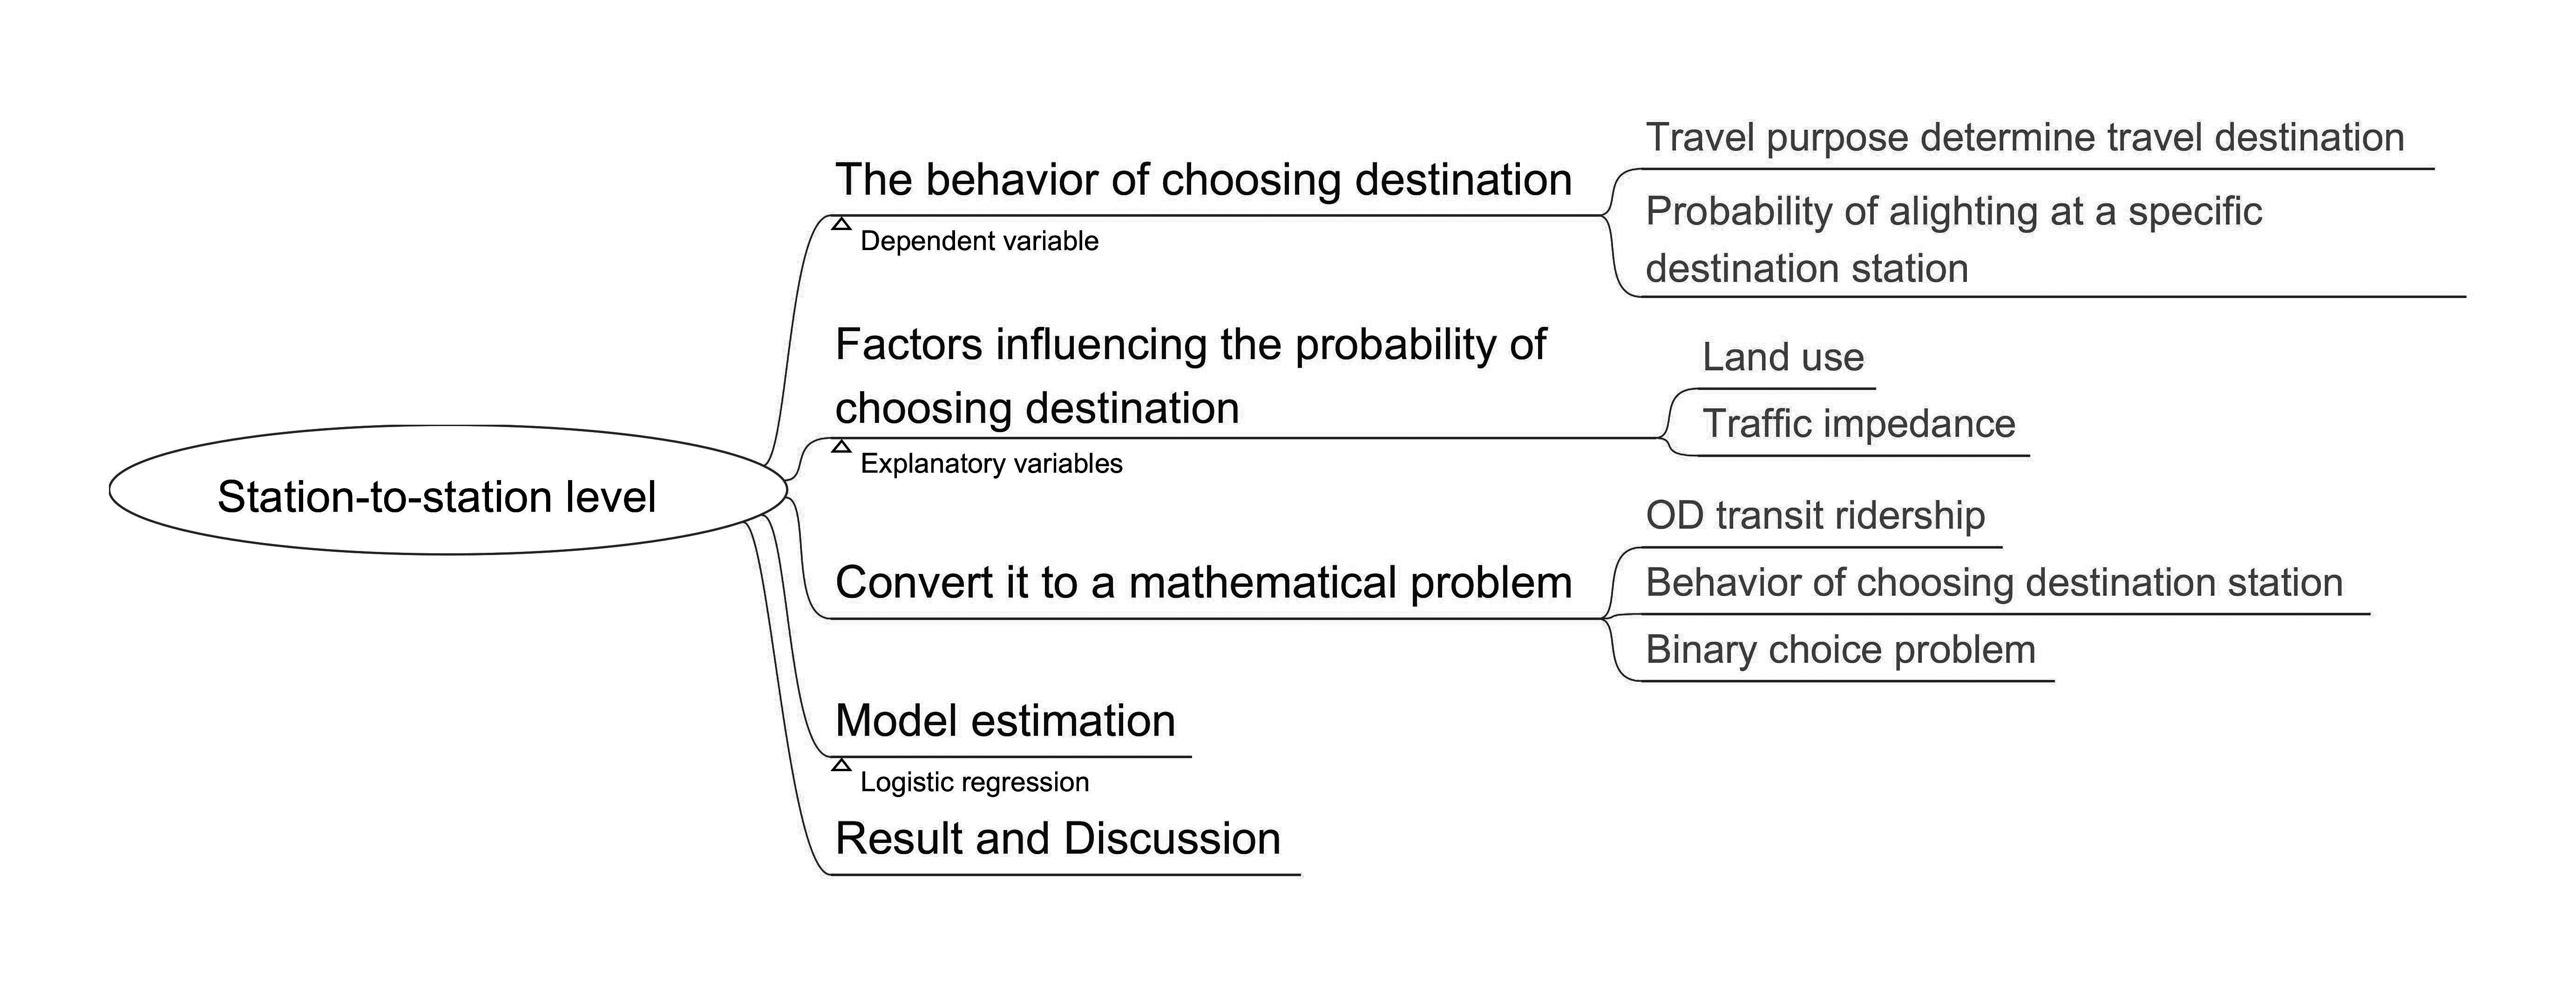
\includegraphics[width=\linewidth]{chapter5/BWChp5Flowchart}
	\caption{Research flowchart}
	\label{fig:chp5:Chp5Flowchart}
\end{sidewaysfigure}

%
\section{Data}

%
\subsection{Case introduction}
%
This study focuses on 35 subway stations in Fukuoka City (the sixth largest city in Japan) which has the largest population in Kyushu Island of Japan (more than 1.5 million). Referring to Figure \ref{fig:chp4:ResearchArea}, the research area and the distribution of subway stations. Until now Fukuoka has three operating subway lines, a total of 29.8 kilometers operating mileage. The transport system carries a daily average of more than 0.6 million passengers by 2015 that accounting for more than 20\% in total motorized travel (from Fukuoka City Transportation Bureau). Although the Fukuoka subway system is not a large-scale one, it plays a crucial role in public transportation in terms of the city scale and population. Moreover, one thing should be noted that the third line is not directly connected with the first and second line. The catchment area of transit stations used in this chapter is the same with that in Chapter 3 (refer to Figure \ref{fig:chp3:BufferAreas}). An 800-meter real walking distance on the road network is used as the pedestrian catchment area. The factors considered to have influences on the passengers' choices for destination stations are described as follow.

%
\subsection{Land-use factors}
%
Land-use is generally accepted as one of the determinants for transit ridership. The indicator of floor area in different building functions can be considered as a detailed expression for land-use. Also, many researchers have verified the influence of floor area in different building functions on transit ridership by conducting empirical studies \cite{sohn2010factors,gutierrez2011transit,chakraborty2013land,chakraborty2013land,jun2015land}. Also, all the stations in the network are connected, the change of land-use within the PCA of a station will lead to the changes of transit ridership in all the stations in the same network. For the case of Fukuoka, about 90\% of the trips accessing subway stations are non-motorized, in another word, the land-use within the PCA of stations play a crucial role in determining the trip purposes of subway users. The accessing duration refers to Table \ref{tab:chp4:AccessToStations}.

%
The same with previous studies, this study chose several types of land-use with higher proportion to assess the indicator of land-use mix, including residential, office, commercial, education. The four main types of land-use account for about 85\% of all the floor area in Fukuoka City, especially in subway PCA, reaching more than 90\%, which refers to Table \ref{tab:chp4:ProportionOfLanduse}. In addition to the indicator of floor area, the index of the land-use mix is also assumed to be a crucial factor for explaining the connectivity of stations \cite{badoe2000transportation,cervero2004transit,frank2004obesity}. Different from the general definition of land-use mix, this study redefines it into the aggregation of land-use. The Euclidean Metric is used for evaluating the deviation of land-use aggregation in each subway station with respect to a reference value. The value of this indicator is ranged from 0 to 1, in which the lower value represents a higher diversity in land-use function, while the higher value means the land-use function is less diverse. This indicator of land-use aggregation is defined as for Equation \ref{eq:chp4:LanduseAggregation}, it is speculated to have a negative impact on ridership. To describe the mixture of land-use closer to the facts, the referenced balance proportion of land-use types is decided by the average proportion of all subway station PCA (800 meters) in Fukuoka City (refer to Table \ref{tab:chp4:ProportionOfLanduse}). There are five variables of land-use category selected as the indicator in this study, the list of indicators also the statistical descriptions refer Table \ref{tab:chp5:StationToStationFactorStatistics}.

% Table
\begin{table}[htbp]
	\centering
	\caption{Summary of the land-use proportion}
	\label{tab:chp5:StationToStationFactorStatistics}%
	\small
	\renewcommand{\arraystretch}{1.25} % 重设表间距
	\begin{tabular}{llrp{5em}<{\raggedleft}p{5em}<{\raggedleft}p{5em}<{\raggedleft}} 
		\Xhline{1.5pt}
		Category & Variable & Unit & Min Value & Max Value & Average \\
		
		\midrule
		\multirow{4}[0]{*}{Land-use}
		& Commerce & \% & 1.03 & 44.58 & 9.89 \\
		& Office & \% & 0.41 & 44.19 & 12.78 \\
		& Residence & \% & 7.15 & 92.26 & 60.34 \\
		& Education & \% & 0.03 & 48.02 & 7.08 \\
		& Land-Use Aggregation & - & 0.09 & 0.75 & 0.31 \\
		
		\Xhline{0.5pt}	
		\multirow{2}[0]{*}{Impedance} 
		& Bus Capacity & - & 58.48 & 2.91 & 259.80 \\
		& Bus Accessibility & - & 89.71 & 4.00 & 455.00 \\
		& Operation Distance & $km$ & 154.50 & 389.30 & 237.58 \\
		\Xhline{1.5pt}
		
	\end{tabular}%
\end{table}%

%
\subsection{Impedance factors}
%
Another factor generally used for representing the connectivity between stations is the remoteness, which is also widely adopted as impedance in the gravity model for explaining the connectivity between traffic zones \cite{iwanow2007trade,kepaptsoglou2010gravity,nitsch2000national}. Impedance is the index that represents the connectivity and cost between origin and destination, it can affect the choice of the trip in terms of both destination and travel mode. Generally, the factor of impedance can be considered from two aspects in this issue, one is the internal impedance that representing the convenience for accessing the station \cite{chu2004ridership,chakraborty2013land}; the other is external impedance that evaluating the connectivity between stations \cite{sohn2010factors}.

%
For Fukuoka, there are about 90\% of all the trip accessing stations by walking and bicycles (refer to Table \ref{tab:chp4:AccessToStations}). Because the PCA is set by the pedestrian distance, the internal road impedance has been already considered in the phase of setting the PCA. It can be thought that there is no need to create a new indicator to represent the internal impedance in this case study.

%
Since the focus of this study is the connectivity between stations, it can be assumed that the interconnection between stations in a subway network is an influential factor in determining the ridership between stations. Two types of external impedance are considered in this study. The operation distance of subway line between two stations is the direct indicator representing the spatial connectivity between two stations. And the impedance of competing modes is also considered in this study. Two indicators of bus accessibility and bus capacity are proposed referring to Equation \ref{eq:chp4:BusCapacity} and Equation \ref{eq:chp4:BusAccessibility} respectively. The former one is used for representing the convenience for accessing the station which is speculated as a positive factor for ridership, while the later one is the transport capacity of the bus within the PCA of the station which is considered as a negative factor for ridership because it may share part of ridership from the subway. All the statistical description of indicators in this study are listed in Table \ref{tab:chp5:StationToStationFactorStatistics}.

%
\section{Methods}
%
\subsection{Flow of the method}
It is difficult to analyze the connectivity of all the stations simultaneously. To simplify this issue, the study will be started by one single station, and then the connectivity between this station and all the other stations connected to it will be investigated. For a passenger, the behavior of going to some places by subway can be viewed as a procedure of choice. In this selection process, the choice is decided by the trip purpose of the passenger. As stated in the introduction, the type of building functions can be mainly categorized into residence, office, education, and commerce, which represent the trip purposes of going home, business, commute, and leisure respectively. Therefore, this issue can be converted into a discrete choice model, in which the dependent variables are the building environment in the station catchment area, and the independent variable is the choice of the destination station.

%
\subsection{Logistic regression}
Taking one station as the destination station, it will correspond to the other departure stations in the subway system. The passengers from the all the departure stations have two options at that destination station, that is getting off and not getting off at this destination station. This probability of getting off at that destination station can be viewed as the representation of the connectivity between the departure station and the destination station. At this point, this issue has been converted into a binary choice problem that investigating the probability of getting off at one subway station. Thus, the Binary-Logistic Regression is introduced into this study to deal with this issue. Formula \ref{eq:chp5:LogisticRegression} shows the Binary-Logistic Regression that will be adopted in the next section.

% Equation 4
\begin{equation}
	p_i(y_i=1 \mid X_i)=\frac{1}{1+e^{-(\alpha +X_i)}}
	\label{eq:chp5:LogisticRegression}
\end{equation}

\begin{description}
	\setlength{\parskip}{0\baselineskip} % 设置段间距
	\normalsize
	\item[\textbf{Where:}]
	\item[$p_i$] is the probability of getting off the subway for the $i$th passenger.
	\item[$y$] is the choice of passengers.
	\item[$X_i$] is the attribute vector of the $i$th passenger.
	\item[$\alpha$] is the residual item
	\setlength{\parskip}{0.7\baselineskip} % 设置段间距
\end{description}

%
For the estimation of a regression model, the model of logistic regression built in this study is a non-linear regression model, which can be directly estimated by using maximum likelihood estimation (MLE). Thus, the MLE is adopted to estimate the coefficient. In this study, the sample size is the passenger volume of all the departure stations connected to the investigated destination station, which is marked as $N$. The same with Equation \ref{eq:chp5:LogisticRegression}, $p_i$ is the probability for choosing to get off, thus, $1-p_i$ represent the probability for choosing not to get off. Then the occurrence probability $L(\theta)$ in all observation sample can be expressed as Equation \ref{eq:chp5:MLE}:

% Equation 5
\begin{equation}
	L(\theta)=\prod_{i=1}^{N}{p_i}^{y_i}(1-p_i)^{(1-y_i)}
	\label{eq:chp5:MLE}
\end{equation}

\begin{description}
	\setlength{\parskip}{0\baselineskip} % 设置段间距
	\normalsize
	\item[\textbf{Where:}]
	\item[$p_i$] is the probability of getting off at the investigated destination station for the $i$th passenger.
	\item[$y_i$] is the choice of $i$th passenger, of which $y_i = 1$ means getting off at the investigated destination station, $y_i = 0$ means not getting off at the investigated station.
	\item[$N$] is the number of passengers riding rail transit at all the departure stations connected to the investigated destination station
	\setlength{\parskip}{0.7\baselineskip} % 设置段间距
\end{description}

\section{Results}
%
The characteristic of land-use within the PCA of a station can represent the characteristic of passengers departing from that station. Since a city is the collection of different functional regions, the land-use characteristics of each PCA are also different. To explore the connectivity between stations with different types of land-use characteristics, this study firstly classifies all the stations in terms of the proportion of different function of land-use and population density. Then the typical stations are chosen from each group of different land-use type, thereby estimating the connectivity between stations by conducting the logistic regression. 

\subsection{Selection of object station}
%
As the result, all the stations are fallen into six categories, they are medium-density residence, high-density residence, education, office, commerce, and airport (refer to Figure \ref{fig:chp3:StationClassification}). Detailed statistics for each type is shown in Table \ref{tab:chp5:StationClassification}, the average values of attributions in each group are represented, furthermore, the factors of bus service and land-use aggregation are also put in this table to help to observe the difference among groups. As is shown, both the group of medium-density residence and the group of high-density residence have a higher proportion of residence floor area, but there is a significant difference in the population density in the two groups. It is clearly that the education type has the highest proportion of education floor area. Both the office type and the commerce type have a higher proportion in office than other types, but the commerce proportion in commerce type is also higher than other types. Additionally, the station of Fukuoka airport does not belong to any group, which mainly takes the feeder traffic from the airport to urban area. It also can be noted that the residence and office type have a relatively lower land-use aggregation and higher population density.

% Table 3
\begin{sidewaystable}[htbp]
	\centering
	\caption{Station classification}
	\label{tab:chp5:StationClassification}
	\small
	\renewcommand{\arraystretch}{1.25} % 重设表间距
	\begin{tabular}{p{12em}<{\raggedright}p{4em}<{\centering}p{4em}<{\centering}p{4em}<{\centering}p{4em}<{\centering}p{4em}<{\centering}p{5em}<{\centering}p{5em}<{\centering}p{5em}<{\centering}}
		
		\Xhline{1.5pt}
		Type & Population density & Commerce & Office & Residence & Education & Land-Use Aggregation & Bus Capacity & Bus Accessibility \\
		\midrule
		
		Medium-density residence & 98 & 4\% & 3\% & \cellcolor[rgb]{.8, .8, .8} 83\% & 4\% & 0.34 & 18 & 28 \\
		High-density residence & 173 & 5\% & 7\% & \cellcolor[rgb]{.8, .8, .8} 76\% & 6\% & 0.26 & 51 & 80 \\
		Education & 83 & 5\% & 6\% & 51\% & \cellcolor[rgb]{.8, .8, .8} 22\% & 0.3 & 45 & 52 \\
		Office & 135 & 8\% & \cellcolor[rgb]{.8, .8, .8} 31\% & 49\% & 3\% & 0.18 & 83 & 131 \\
		Commerce & 69 & \cellcolor[rgb]{.8, .8, .8} 34\% & \cellcolor[rgb]{.8, .8, .8} 32\% & 24\% & 1\% & 0.47 & 132 & 213 \\
		Airport & 36 & 1\% & 3\% & 45\% & 2\% & 0.23 & 32 & 56 \\
		\Xhline{1.5pt}
		
	\end{tabular}
	%
	\begin{description}
		\small
		\label{note:tab:chp5:StationClassification}
		\item[Note:] the highlighted cells refer to the representative values that having much higher percentage than other land-use types.
	\end{description}
	
\end{sidewaystable}

%
To investigate the stations with significant differences in land-use characteristic, the most typical object station is chosen from each group in terms of the guidelines as follow: 

\begin{itemize}
	\item Avoid selecting the stations with the highest value of feature indicator. Because the high value may be caused by the particularity of its distribution of land-use and road network, it does not have generality in terms of the type it is.
	\item Avoid selecting the transferable stations. Because the transit ridership of this kind of stations generally relates the other stations, which cannot reflect the distribution of land-use within the PCA.
	\item Avoid selecting the stations with much lower or higher population density than other stations. Because the low or high population density may lead to different travel preference due to the difference in the distribution of facilities (such as hospitals, schools, and transportation facilities etc.).
	\item Finally, six stations are selected from six groups, the factor of each station is shown in Table \ref{tab:chp5:Result}.
\end{itemize}

% Table 4
\begin{sidewaystable}[htbp]
	\centering
	\caption{Result of Logistic Regression}
	\label{tab:chp5:Result}
	\footnotesize % 该表使用小字体
	\renewcommand{\arraystretch}{1.25} % 重设表间距
	
	\begin{tabular}{p{7em}p{5em}p{5em}<{\centering}rrrrrrrrr}
		\Xhline{1.5pt}
		
		% 表题第一行
		\multicolumn{2}{c}{Destination Station} & & \multicolumn{9}{c}{Variables in Boarding Station} \\
		\midrule
		
		% 表题第二行
		\multirow{2}[5]{7em}{Type} & \multirow{2}[5]{5em}{Station} & \multirow{2}[5]{5em}{\centering{Statistical index}} & \multicolumn{5}{c}{Land-use} & & \multicolumn{3}{c}{Impedance} \\
		\cmidrule{4-8} \cmidrule{10-12}
		
		% 表题第三行
		& & & 
		\multicolumn{1}{p{5em}}{\centering{Commerce}} & 
		\multicolumn{1}{p{5em}}{\centering{Office}} & 
		\multicolumn{1}{p{5em}}{\centering{Residence}} & 
		\multicolumn{1}{p{5em}}{\centering{Education}} & 
		\multicolumn{1}{p{5em}}{\centering{Land-use Aggregation}} & &  \multicolumn{1}{p{5em}}{\centering{Distance}} & 
		\multicolumn{1}{p{5em}}{\centering{Bus Capacity}} & 
		\multicolumn{1}{p{5em}}{\centering{Bus Accessibility}} \\
		\midrule
		
		% 开始表的内容
		\multirow{3}[0]{7em}{Medium-density residence} & \multirow{3}[0]{5em}{Kamo} & \textsl{B} & -0.05 & -0.06 & -0.06 & -0.07 & -0.03 & & 0.07 & 0.01 & -0.01 \\
		& & \textsl{P-value} & 0.00 & 0.00 & 0.00 & 0.00 & 0.00 & & 0.00 & 0.04 & 0.04 \\
		& & \textsl{Exp(B)} & 0.95 & 0.94 & 0.94 & 0.93 & 0.97 & & 1.07 & 1.01 & 1.00 \\
		\midrule
		
		\multirow{3}[0]{7em}{High-density residence} & \multirow{3}[0]{5em}{Fujisaki} & \textsl{B} & 0.01 & \cellcolor[rgb]{.8, .8, .8} 0.00 & -0.01 & 0.01 & -0.02 & & -0.06 & 0.00 & 0.00 \\
		& & \textsl{P-value} & 0.00 & \cellcolor[rgb]{.8, .8, .8} 0.18 & 0.00 & 0.00 & 0.00 & & 0.00 & 0.00 & 0.00 \\
		& & \textsl{Exp(B)} & 1.01 & \cellcolor[rgb]{.8, .8, .8} 1.00 & 0.99 & 1.01 & 0.98 & & 0.95 & 1.00 & 1.00 \\
		\midrule
		
		\multirow{3}[0]{7em}{Education} & \multirow{3}[0]{5em}{Hakozakikyudai} & \textsl{B} & 0.02 & \cellcolor[rgb]{.8, .8, .8} 0.00 & 0.02 & 0.03 & -0.01 & & -0.13 & 0.00 & 0.00 \\
		& & \textsl{P-value} & 0.00 & \cellcolor[rgb]{.8, .8, .8} 0.53 & 0.00 & 0.00 & 0.00 & & 0.00 & 0.04 & 0.00 \\
		& & \textsl{Exp(B)} & 1.02 & \cellcolor[rgb]{.8, .8, .8} 1.00 & 1.02 & 1.03 & 0.99 & & 0.88 & 1.00 & 1.00 \\
		\midrule
		
		\multirow{3}[0]{7em}{Office} & \multirow{3}[0]{5em}{Gofukumachi} & \textsl{B} & 0.02 & -0.02 & 0.02 & 0.05 & -0.01 & & \cellcolor[rgb]{.8, .8, .8} -0.01 & 0.00 & 0.00 \\
		& & \textsl{P-value} & 0.00 & 0.00 & 0.00 & 0.00 & 0.01 & & \cellcolor[rgb]{.8, .8, .8} 0.72 & 0.03 & 0.00 \\
		& & \textsl{Exp(B)} & 1.02 & 0.98 & 1.02 & 1.06 & 0.99 & & \cellcolor[rgb]{.8, .8, .8} 0.99 & 1.00 & 1.00 \\
		\midrule
		
		\multirow{3}[0]{7em}{Commerce} & \multirow{3}[0]{5em}{Tenjinn} & \textsl{B} & -0.01 & -0.01 & 0.01  & 0.03  & 0.02  & & 0.06 & \cellcolor[rgb]{.8, .8, .8} 0.00 & 0.00 \\
		& & \textsl{P-value} & 0.00 & 0.00 & 0.00 & 0.00  & 0.00 & & 0.00 & \cellcolor[rgb]{.8, .8, .8} 0.38 & 0.00 \\
		& & \textsl{Exp(B)} & 1 & 0.99 & 1.01 & 1.03 & 1.02 & & 1.06 & \cellcolor[rgb]{.8, .8, .8} 1.00 & 1.00 \\
		\midrule
		
		\multirow{3}[0]{7em}{Airport} & \multirow{3}[0]{5em}{Fukuoka Airport} & \textsl{B} & -0.03 & 0.03 & -0.01 & -0.02 & 0.03 & & -0.08 & 0.00 & 0.00 \\
		& & \textsl{P-value} & 0.00 & 0.00 & 0.00 & 0.00 & 0.00 & & 0.00 & 0.00 & 0.00 \\
		& & \textsl{Exp(B)} & 0.97 & 1.03 & 0.99 & 0.99 & 1.03 & & 0.92 & 1.00 & 1.00 \\
		\Xhline{1.5pt}
		
	\end{tabular}%
%
	\begin{description}
		\footnotesize
		\label{note:tab:chp5:Result}
		\item[Note:]
		$B$ is the coefficient \\
		$Exp(B)$ is the odds ratio \\
		Gray cell means the estimated value is not significant at the significance level of 0.05 \\
	\end{description}
	
\end{sidewaystable}%

\subsection{Estimation of logistic regression}
%
In this study, the independent variable is the choice of getting off at the object station or not, and the influencing factors are land-use and impedance between stations and stations. Notably, in the case of Fukuoka subway network, subway line 3 is not directly connected with that line 1 and line 2, thus subway line 3 is addressed separately from subway line 1 and line 2. That is, if the object station belongs to subway line 3, the connectivity will be only investigated within subway line 3. The result of estimation is shown in Table \ref{tab:chp5:Result}.

%
The estimation is as shown in Table \ref{tab:chp5:Result}, the values in gray cell mean that this factor showed no statistical significance at the confidence level of 0.05. The index of $Exp(B)$, which is the odds ratio, represents the extent to the effect on the probability of choice if the coefficient $B$ changes one unit. Here giving a brief explanation of the index of $Exp(B)$, since the unit and meaning of the variables entered the models are different. For the variables of land-use, the index of $Exp(B)$ represents that the 1 percent (0.01 unit) change in the variables will lead to an $Exp(B)$ multiples of increases in the probability of getting off at the object station. For the variables of impedance, it means the 1 unit change in the variables will lead to an $Exp(B)$ multiples of increases in the probability of choosing the object station as a destination. 

%
A further explanation taking the Tenjin station as an example is given as below. From the point of land-use, the increase of commerce and office floor area in the catchment area of the boarding stations can lead to a decrease in the probability of choosing the Tenjin station as the destination station; while the increase of residence and education floor area in the catchment area of boarding stations can raise the probability of choosing to go the Tenjin station. If interpreted in terms of connectivity, the business type of Tenjin Station is weakly connected to stations with the same commercial type, and the stations of office type; while the stations of business type have relatively strong connectivity with the stations of residence and education type. 

%
\section{Discussion}
%
From the perspective of TOD, this study investigated the connectivity between stations with different land-use characteristic by examining the impact of land-use and impedance on subway passengers' choice of the destination station. As shown in Table \ref{tab:chp5:StationClassification}, the PCA of the station in Fukuoka shows a significant characteristic of land-use distribution, and all the subway stations are categorized into six major types. The result of logistic regression shows the coefficient of factor influencing the choice of the destination station, which can be explained as the connectivity between different PCAs.

%
Some findings of the land-use factors can be known from the result in Table \ref{tab:chp5:Result}. The increase in the proportion of residence area of the departure station can lead to an increase in the choice of taking the office and education type station as destination stations. This can be explained as the result of commuter traffic since there is a relatively stronger connectivity between the residential area and work area \cite{badoe2000transportation}. But the situation may change in the medium-residence type due to the different travel preferences in the area with different population density. Another interesting finding is that all kinds of land-use have positive connectivity with the education type station. One speculation is that students tend to take public transit because of the low income. Overall, one kind of land-use generally shows a rejection effect on the station which has a similar consist of land-use type. Such as the Tenjin station located in the CBD area, the proportion of commerce area in the PCA of departure station causes a negative effect on the choice of getting off at Tenjin station. Moreover, the variable of land-use aggregation shows that there is a positive connectivity between the areas with an unbalanced distribution of land-use.

%
The factors of impedance also showed a good statistical significance, however, the results do not seem to show a certain regularity in different types of stations. Here some possible speculations of the reasons are given for helping to find the limitation of this study and explore the direction for the next study. First, the share of different transportation modes is not considered in this study. The distance between two stations may also affect the variation in the share of different transportation modes, thus it is not stable in representing the impedance.  Second, the variables of bus service describe the features of one single station, but not the features that reflecting the connectivity between two stations. If considering two stations, one is in the downtown where the transportation hub locates, and one is in suburban where there are few public transportation facilities; it can be inferred that even though the bus service is rich in the downtown area, it affects very little on the station located in the suburban area.

%
\section{Conclusion}
%
This study investigated the effect of land-use and impedance between stations on the OD subway ridership from the perspective of the connectivity. The effect of factors on the choice of destination station was estimated using the logistic regression model. The result showed that the influence of land-use on the ridership between stations was effective, and this result could be explained consistently with fact; while the factor of impedance was still difficult to get explained.

%
From the results obtained in this article, in the urban rail transit, the land-use within the station catchment area is an important factor in determining the destination of passengers. Correspondingly, the change in the choice of destination can be reflected to the transit ridership. Furthermore, this change in the transit ridership of each station, which is caused by the change in the choice of destination, is the reflect of the connectivity between the station and the station in terms of land-use in each station catchment area. The results are clearly shown in Table \ref{tab:chp5:Result}.

%
Based on the results in this study, the next stage of this research will focus on the share ratio in different transportation modes to make a deeper exploration of subway ridership. The factor of impedance will also be rebuilt to help to describe the connectivity between stations more accurately.

% reference
\clearpage % 新起一页
\bibliographystyle{apacite}
% \bibliographystyle{IEEEtran}
\bibliography{ref}